\documentclass[a4paper,12pt]{article} % declaration
\usepackage[utf8]{inputenc}
\usepackage{amsmath}
\usepackage{amssymb}
\usepackage{amsfonts}
\usepackage{color}
\usepackage{enumitem}
\usepackage{graphicx}
\usepackage{fancyhdr}
\usepackage{color}
\usepackage{amsthm}

%\def\pgfsysdriver{pgfsys-dvipdfmx.def}
\usepackage{tikz}

\newtheorem{definition}{Definition}[section]
\newtheorem{example}{Example}[section]
\newtheorem{theorem}{Theorem}[section]
\newtheorem{proposition}{Proposition}[section]
\newtheorem{lemma}[theorem]{Lemma}
\newtheorem{corollary}[theorem]{Corollary}

\title{Introduction}
\author{Guoning Wu}

\begin{document}
\graphicspath{{../Figs/}}

%\tableofcontents
\setcounter{tocdepth}{2}

%\listoffigures
%\listoftables

\maketitle

In this note, we introduce some basic concepts for real 
analysis.

\section{Sets and Elementary Operations on them}
\subsection{The Concept of a Set}
Since the late nineteenth and early twentieth centuries 
the most universal language of mathematics has been the 
language of set theory. This is even manifest in one of 
the definitions of mathematics as the science that 
studies different structures (relations) on sets.

\emph{"We take a set to be an assemblage of definite, 
perfectly distinguishable objects of our intuition or 
our thought into a coherent whole."} Thus did Georg 
Cantor\footnote{G.Cantor(1845-1918) - German 
mathematician, the creator of the theory of infinite 
sets and the progenitor of set theoretic language in 
mathematics.}, describe the concept of a set.

\begin{itemize}
    \item A set may be consist of any distinguishable 
        objects.
    \item A set is unambiguously determined by the 
        collection of objects that comprise it.
    \item Any property defines the set of objects 
        having that property.
\end{itemize}

If $x$ is an object, $P$ is a property, and $P(x)$ 
denotes the assertion that $x$ has property $P$, 
then the class of objects having the property
$P$ is denoted $\{x\lvert P(x)\}$

And in fact the concept of the set of all sets, for 
example, is simply contradictory. This is the 
classical paradox of \textbf{Russell}. \footnote{B.Russell (1872-1970) - British logician,
philosopher, sociologist ans social activist.}

\subsection{The Inclusion Relation}
The statement, "$x$ is an element of the set $X$" is written 
briefly as
\[ 
    x\in X
\]
and its negation as
\[
    x \notin X
\]

When statements about sets are written, frequent use is 
made of the logical operators $\exists$ ("there exists" or "there
are") and $\forall$ ("every" or "for all") which are called the
\emph{existence} and \emph{generalization} respectively.

Thus two sets are equal if they consist of the same 
elements, this statement is usually written briefly as 
\[
    A=B,
\]
read as "$A$ equals $B$". The negation of equality is usually 
written as 
\[
    A \ne B.
\]
If every element of $A$ is an element of $B$, we write
$A\subset B$ and say that $A$ is a subset of 
$B$ or that $B$ contains $A$.

Thus 
\[
    A\subset B := \forall x\in A \Rightarrow x\in B
\]
If $A\subset B$ and $A\ne B$, we shall say that the inclusion $A\subset B$ is 
\emph{strict} or that $A$ is a proper subset of $B$.

Using these definitions, we can now conclude that
\[A=B \Leftrightarrow A\subset B \wedge B\subset A\]
If $M$ is a set, any property of $P$ distinguishes in M the subset
\[\{x\in M \vert P(x)\}\]
consisting of the elements of $M$ that have the property.

For example, it is obvious that 
\[ M=\{x\in M \vert x\in M\},\]
and the \emph{empty} subset of $M$ is 
\[\emptyset = \{x\in M \vert x\ne x\}\]

\subsection{Elementary Operations on Sets}
\begin{figure}[htbp]
    \centering
    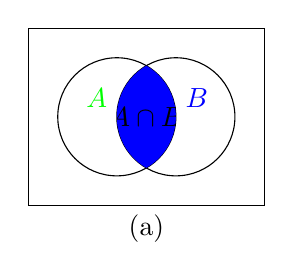
\begin{tikzpicture}[scale=0.75]
    \draw  (0,0) rectangle  (4,3);
        \node [below,black] at (2, 0) {(a)};
    \draw (2.5,1.5) circle (1);
    \draw (1.5,1.5) circle (1);
    \node [above left,green] at (1.5, 1.5) {$A$};
    \node [above right,blue] at (2.5, 1.5) {$B$};
    \clip (1.5,1.5) circle (1);
    \clip (2.5,1.5) circle (1);
    \draw [fill, blue!100] (0, 0) rectangle (4, 3);
    \node [black] at (2, 1.5) {$ A\cap B$};
\end{tikzpicture}
    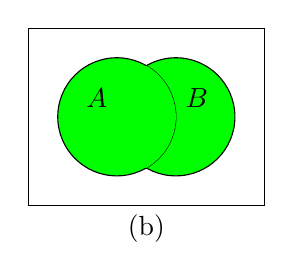
\begin{tikzpicture}[scale=0.75]
    \draw  (0,0) rectangle  (4,3);
        \node [below,black] at (2, 0) {(b)};
    \draw [fill=green](2.5,1.5) circle (1);
    \draw [fill=green] (1.5,1.5) circle (1);
    \node [above left,black] at (1.5, 1.5) {$A$};
    \node [above right,black] at (2.5, 1.5) {$B$};
    \clip (1.5,1.5) circle (1);
    \clip (2.5,1.5) circle (1);
    \draw [fill, green] (0, 0) rectangle (4, 3);
\end{tikzpicture}
    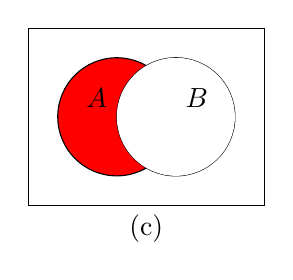
\begin{tikzpicture}[scale=0.75]
    \draw  (0,0) rectangle  (4,3);
        \node [below,black] at (2, 0) {(c)};
    \draw [fill=red](1.5,1.5) circle (1);
    \draw (2.5,1.5) circle (1);
    \node [above left,black] at (1.5, 1.5) {$A$};
    \clip (0,0) rectangle  (4,3);
    \clip (2.5,1.5) circle (1);
    \draw [fill,black!0] (0, 0) rectangle (4, 3);
    \node [above right,black] at (2.5, 1.5) {$B$};
\end{tikzpicture}
    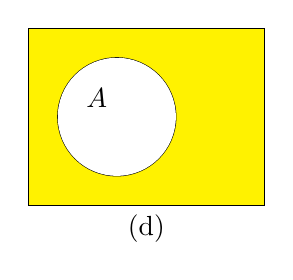
\begin{tikzpicture}[scale=0.75]
    \draw [fill=yellow] (0,0) rectangle  (4,3);
        \node [below,black] at (2, 0) {(d)};
    \draw (1.5,1.5) circle (1);
    \clip (1.5,1.5) circle (1);
    \draw [fill,yellow!0] (0, 0) rectangle (4,3);
    \node [above left,black] at (1.5, 1.5) {$A$};
\end{tikzpicture}
\label{sets}
    \caption{(a) Intersection. (b) Union. (c) Difference. (d) Complement. }
\end{figure}

Let $A$ and $B$ be subsets of a set $M$.
\begin{enumerate}[label={\rm (\alph*)}]
    \item The {\color{red}\textbf{union}} of $A$ and $B$ is the set 
        $\displaystyle A \cup B \triangleq \left\{ x \in M \vert x \in A \vee x \in B \right\}$
    \item The {\color{red}\textbf{intersection}} of $A$ and $B$ is the set 
        $\displaystyle A \cap B \triangleq \left\{ x \in M \wedge x \in A \vee x \in B \right\}$
    \item The {\color{red}\textbf{difference}} of $A$ and $B$ is the set 
        $\displaystyle A \setminus B \triangleq \left\{ x \in M \vert x \in A \vee x \notin B \right\}$
    \item The {\color{red}\textbf{direct(Cartesian) product of sets.}}
        For any two sets $A$ and $B$ one can form a new set, namely 
        the pair $\left\{A, B\right\} = \left\{B, A\right\}$, which consists of the sets 
        $A$ and $B$ and no others.This set has two elements if $A \ne B$ and 
        one element if $A = B.$
        This set is called the unordered pair of sets $A$ and $B$, to 
        be distinguished from the ordered pair $(A, B)$ in which 
        the elements are endowed with additional properties to 
        distinguish the first and the second elements of the pair 
        $\left\{A, B\right\}$. The equality 
        \[
            (A, B) = (C, D)
            \]
        between two ordered pairs means by definition that $A = C$ 
        and $B = D$. In particular, if $A \ne B$, then $(A, B) \ne (B, A)$.

        Now let $X$ and $Y$ be arbitrary sets. The set 
        \[
            X \times Y \triangleq \left\{(x, y) \vert (x \in X) \wedge (y \in Y) \right\}
            \]
        formed by the ordered pairs $(x, y)$ whose first element belongs 
        to $X$ and whose second element belongs to $Y$, is called the 
        {\color{red} Cartesian product} of the set $X$  and $Y$.
\end{enumerate}

\section{Functions}
\subsection{The Concept of a Function (Mapping)}
The term \textit{function} first appeared in the years from 1673 to 1692 in
works of G.Leibniz. By the year 1698 the term had become established
in a sense close to the modern one through the correspondence 
between Leibniz and Johann Bernoulli.
\footnote{Johann Bernoulli (1667-1748) - one of the early representatives
of the distinguished Bernoulli family of Swiss scholars, he studied 
analysis, geometry and mechanics. He was one of the founders of the 
calculus of variations. He gave the first systematic exposition of 
the differential and integral calculus.}

Let $X$ and $Y$ be certain sets. We say that there is a function defined 
on $X$ with values in $Y$ if, by virtue of some rule $f$, to each element 
$x \in X$ there corresponds an element $y \in Y$. In this case the set $X$
is called the {\color{red} \textbf{domain}} of the function.
The symbol $x$ used to denote a general element of the domain is 
called the argument of the function. The element $y_0 \in Y$ corresponding 
to a particular value $x_0 \in X$ is called the value of the function 
at $x_0$, and is denoted as $f(x_0)$. As the argument $x \in X$ varies, the value
$y = f(x) \in Y$, in general, varies depending on the values of $x$.
For that reason, the quality $y = f(x)$ is often called the dependent 
variable.

The set 
\[
    f(X) = \left\{y \in Y \vert \exists x, x \in X \wedge y = f(x) \right\}
\]
of values assumed by a function on elements of the set $X$ will 
be called the set of values or the range of the function.

For a function the following notations are standard:
\[
    f: X \to Y,  X \xrightarrow{f} Y
    \]

Two functions (mapping) $f_1$ and $f_2$ are identical or equal 
if the have the same domain $X$ and each element $x \in X$ the values 
$f_1(x)$ and $f_2(x)$ are the same. In this case we write $f_1 = f_2$.

\begin{example}
    The formulas $l = 2\pi r$ and $V = \frac{4}{3}\pi r^3$ establish 
    functional relationships between the circumference $l$
    of a circle and its radius $r$ and between the volume $V$
    of a ball and its radius $r$. Each of these formulas provides 
    a particular function $f: \mathbb{R}_+ \to \mathbb{R}_+$
    defined on the set $\mathbb{R}_+$ of the positive real numbers 
    with values in the same set.
\end{example}

\begin{example}
    The mapping $G: \mathbb{R}^2 \rightarrow \mathbb{R}^2$ (the direct product 
    $\displaystyle \mathbb{R}^2 = \mathbb{R} \times mathbb{R} = \mathbb{R}_t 
    \times \mathbb{R}_x$) into itself defined by the foumulas:
    \[
    \begin{array}{ll}
        x' & = x - vt \\
        t' & = t
    \end{array}
    \]
   is the classical Galilean transformation for transition from 
    one inertial coordinate system $(x,t)$ to another system $(x', t')$
    that is in motion relative to the first speed $v$.

    The same purpose is served by the mapping $L: \mathbb{R}^2 
    \to \mathbb{R}^2$ defined by the relations:
    \[
    \begin{array}{ll}
        x' = \frac{x - vt}{\sqrt{1 - \left(\frac{v}{c}\right)^2}},\\
        t' = \frac{t - \frac{v}{c^2}x}{\sqrt{1-\left(\frac{v}{c}\right)^2}}
     \end{array}
     \]
     is the well known (one-dimensional) Lorentz transformation,
     which play a fundamental role in the special theory of
     relativity. The speed $c$ is the speed of light.
\end{example}

\begin{example}
    The projection $pr_1: X_1 \times X_2 \to X_1$ and $pr_2: X_1 \times X_2 \to X_2$
    are obvious functions.
\end{example}

\subsection{Elementary Classification of Mapping}
A mapping $f: X \to Y$ is said to be 

{\color{red} surjective} if $f(X) = Y$;

{\color{red} injective} if for any elements $x_1, x_2 \in X$
\[
    f(x_1) = f(x_2) \Rightarrow x_1 = x_2
    \]

{\color{red} bijective} if it is both surjective and injective.

\subsection{Some Special Functions}
\begin{example}{The absolute value function}
    \[
        \left|x\right| = \left\{ \begin{array} {cc}
                          x, & x \ge 0 \\
                         -x, & x < 0
        \end{array}\right.
        \]
\end{example}

\begin{figure}[h!]
    \centering
    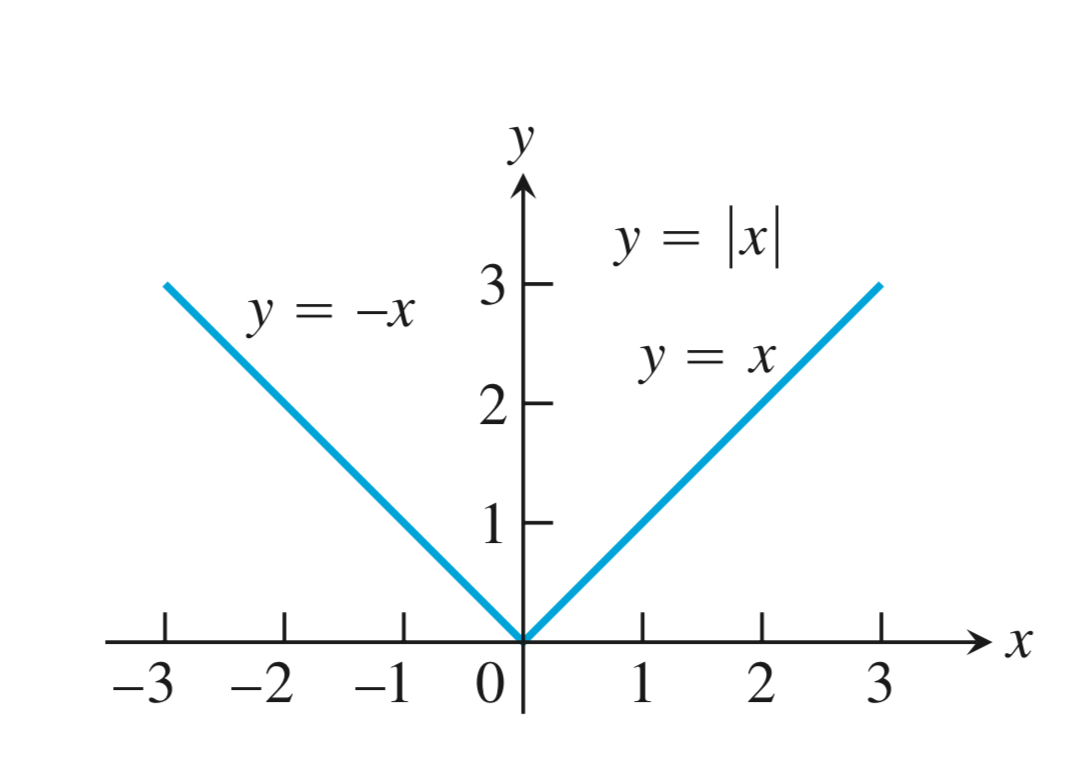
\includegraphics[width=0.5\textwidth]{absolutefun.png}
    \caption{The absolute function.}
    \label{fig:absolutefun}
\end{figure}

\begin{example}{The Greatest Integer Function}
    This function whose value at any number $x$ is the greatest 
    integer less than or equal to $x$ is called the greatest 
    integer function or the integer floor function. It is 
    denoted as $\lfloor x \rfloor$
\end{example}
\begin{figure}[h!]
    \centering
    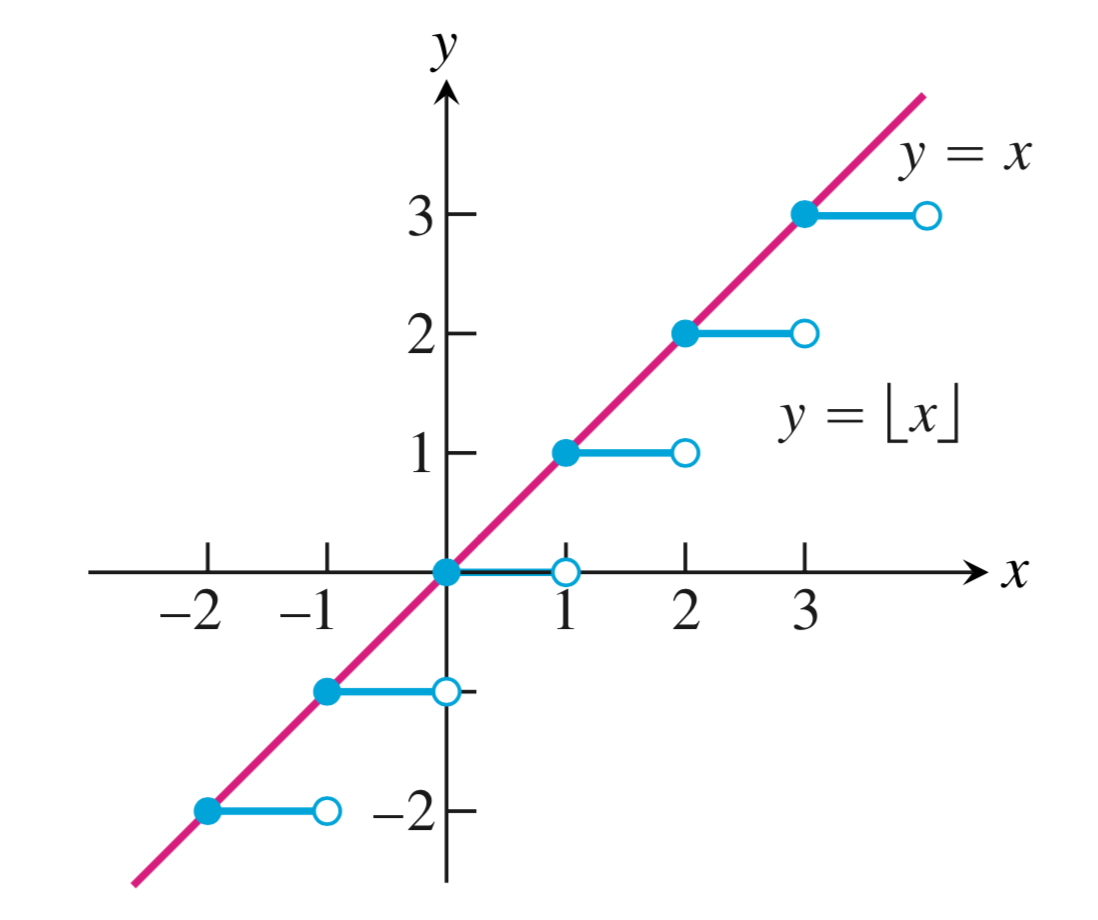
\includegraphics[width=0.5\textwidth]{gintfun.png}
    \caption{The greatest integer function.}
    \label{fig:gintfun}
\end{figure}

\begin{example}{The Least Integer Function}
    This function whose value at any number $x$ is the smallest 
    integer great than or equal to $x$ is called the leastest 
    integer function or the integer ceiling function. It is 
    denoted as $\lceil x \rceil$
\end{example}
\begin{figure}[h!]
    \centering
    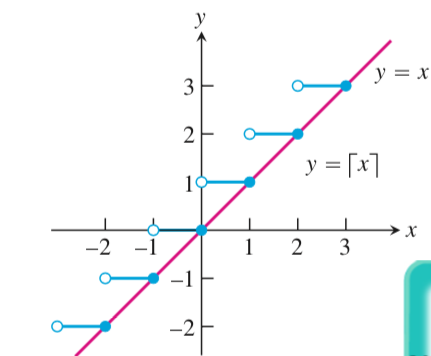
\includegraphics[width=0.5\textwidth]{lintfun.png}
    \caption{The least integer function.}
    \label{fig:lintfun}
\end{figure}

\begin{example}{The Sign Function or Signum Function}
    The signum function of a real number $x$ is defined as 
    follows:
    \[
        \rm{sgn} (x) = \left\{\begin{array}{cc} 
                   -1,  & x < 0\\
                    0,  & x = 0\\
                    1,  & x = 1
        \end{array}\right.
        \]
\end{example}

\begin{figure}[h!]
    \centering
    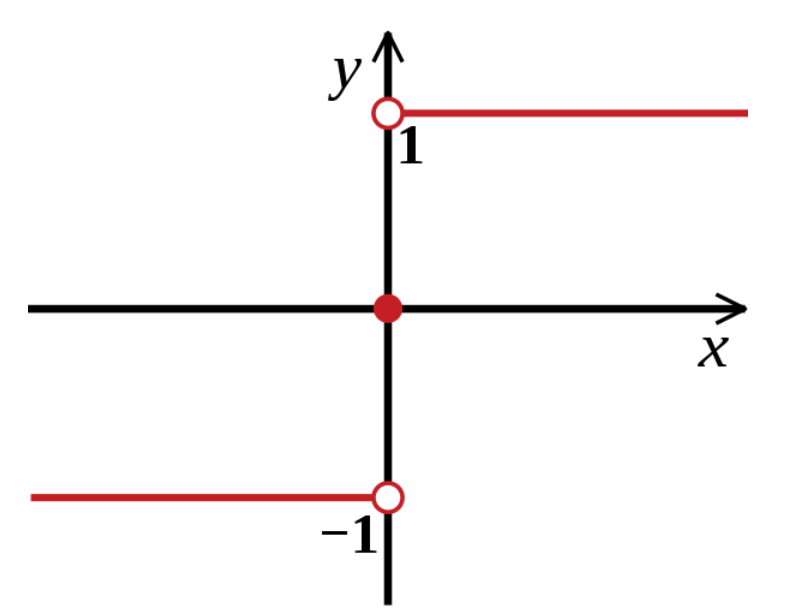
\includegraphics[width=0.5\textwidth]{signumfun.png}
    \caption{The singnum function.}
    \label{fig:singnum}
\end{figure}

\begin{example}{The Dirichlet Function}
    \[
        \rm D(x) = \left\{\begin{array}{cc} 
            1, & x \in \mathbb{Q},\\
            0, & x \in \mathbb{R} \setminus \mathbb{Q}
        \end{array}\right.
        \]
\end{example}

\begin{example}{The Riemann Function}
    \[
        \rm R(x) = \left\{ \begin{array}{cc} 
            \frac{1}{q}, & x = \frac{p}{q}, p, q \in \mathbb{Z}^+, (p, q) = 1\\
                   0,    & x = 0, 1, (0,1) \setminus \mathbb{Q}
        \end{array}\right.
        \]
\end{example}
\begin{figure}[h!]
    \centering
    \includegraphics[width=0.5\textwidth]{rimannfun.pdf}
    \caption{The Rimann function.}
    \label{fig:rimann}
\end{figure}




\section{The Real Numbers}
Numbers in mathematics are like time in physics: everyone knows what 
they are, and only experts find them hard to understand.
\subsection{The Axiom System and some General Properties of the 
Set of Real Numbers}
\begin{definition} {A set $\mathbb{R}$ is called the set of \textit{real numbers}
and its elements are \textit{real numbers} if the following list of conditions
holds, called the axiom system of the real numbers.}
\end{definition}

\begin{center}
    (I) AXIOMS FOR ADDITION
\end{center}
An operation 
\[+:\mathbb{R}\times\mathbb{R} \to \mathbb{R}\]
is defined, assigning to each ordered pair $(x,y)$ of elements 
$x,y$ of $\mathbb{R}$ a certain element $x+y\in\mathbb{R}$, called 
the sum of $x$ and $y$. The operation satisfies the following 
conditions:
\begin{enumerate}
    \item There exists a neutral, or identity element 0 
        (called zero) such that 
    \[x+0=0+x=x\]
    for every $x\in\mathbb{R}$.
    \item For every element $x\in \mathbb{R}$ there exists an element 
    $-x\in\mathbb{R}$ called the negative of $x$ such that
        \[x+(-x)=(-x)+x=0\].
    \item The operation is associative, that is, the relation
        \[x+(y+z) = (x+y)+z\] for any elements of $x,y,z$ of $\mathbb{R}$.
    \item The operation is commutative, that is 
        \[x+y=y+x\] for any elements $x,y$ of $\mathbb{R}$.
\end{enumerate}

If an operation is defined on a set $G$ satisfying axiom 1, 2 and 3, we
say that a group structure is defined on $G$ or that $G$ is a group. 
If the operation is called addition, the group is called an additive 
group. If it is also known that the operation is commutative, that is, 
condition 4 holds, the group is called commutative or \textit{Abelian} is a group. 
If the operation is called addition, the group is called an additive 
group. If it is also known that the operation is commutative, that is, 
condition 4 holds, the group is called commutative or \textit{Abelian}.

\begin{center}
    (II) AXIOMS FOR MULTIPLICATION
\end{center}
An operation \[\bullet:\mathbb{R}\times\mathbb{R}\to\mathbb{R}\]
(the operation of multiplication) is defined, assigning to 
each ordered pair $(x,y)$ of elements of $\mathbb{R}$ a certain
element $x\cdot y\in \mathbb{R}$, called the product of $x$ and 
$y$. This operation satisfies the following conditions:
\begin{enumerate}
    \item There exists a neutral, or identity element 
        $1\in \mathbb{R}\setminus 0$ (called one) such that 
        \[x\cdot 1 = 1\cdot x=x\] for every $x\in \mathbb{R}$
    \item For every element $x\in\mathbb{R}\setminus 0 $ 
        there exists an element $x^{-1}\in \mathbb{R}$ ,
        called the inverse or reciprocal of $x$, such that
        \[x\cdot x^{-1}=x^{-1}\cdot x=1\]
    \item The operation $\bullet$ is commutative, that is 
        \[x\cdot(y\cdot z) = (x\cdot y)\cdot z\] holds 
        for every elements $x,y,z$ of $\mathbb{R}$.
    \item The operation $\bullet$ is commutative, that is 
        \[ x\cdot y = y\cdot x\] for every elements $x,y$ of $\mathbb{R}$.
\end{enumerate}

\begin{center}
    (I, II) THE CONNECTION BETWEEN ADDITION AND MULTIPLICATION
\end{center}
Multiplication is distributive with respect to addition, that
is \[(x+y)z = xz+yz\] for all $x,y,z\in \mathbb{R}$

We remark that if two operations satisfies these axioms 
are defined on a set $G$, then $G$ is called a field.

\begin{center}
    (III) ORDER AXIOMS
\end{center}
Between elements of $\mathbb{R}$ there is a relation $\le$,
that is, for elements $x,y\in\mathbb{R}$ one can determine 
whether $x\le y$ or not. Here the following conditions must 
hold:
\begin{enumerate}
    \item $\forall x\in \mathbb{R}(x\le x)$
    \item $(x\le y)\wedge (y\le x) \Rightarrow (x=y)$
    \item $(x\le y) \wedge(y\le z) \Rightarrow (x\le z)$
    \item $\forall x\in \mathbb{R} ,\forall y\in \mathbb{R} (x\le y) \vee (y\le x)$
\end{enumerate}

\begin{center}
    (I, III) THE CONNECTION BETWEEN ADDITION AND ORDER ON $\mathbb{R}$
\end{center}
If $x,y,z$ are elements of $\mathbb{R}$, then 
\[(x\le y) \Rightarrow (x+z) \le (y+z)\]

\begin{center}
    (II, III) THE CONNECTION BETWEEN MULTIPLICATION AND 
    ORDER ON $\mathbb{R}$
\end{center}
If $x$ and $y$ are elements of $\mathbb{R}$, then
\[(0\le x)\wedge(0\le y) \Rightarrow (0\le x\cdot y)\]

\begin{center}
    (IV) THE AXIOM OF COMPLETENESS (CONTINUITY)
\end{center}
If $X$ and $Y$ are nonempty subsets of $\mathbb{R}$ having 
the property that $x\le y$ for every $x\in X$ and every $y\in Y$,
then there exists $c\in\mathbb{R}$ such that $x\le c \le y$  for 
all $x\in X$ and $y\in Y$.

We now have a complete list of axioms such that any set on 
which those axioms hold can be considered a concrete 
realization or model of the real numbers.

\subsection{The Most Important Classes of Real Numbers}
\subsubsection{The Natural Numbers and the Principle of Mathematical 
Induction}
\begin{definition} 
    The numbers of the form $1,1+1,(1+1)+1,$ and so forth are denoted 
    respectively by $1,2,3,\cdots$ and so forth and are called natural
    numbers.
\end{definition}
\begin{definition}
    A set $X\subset\mathbb{R}$ is inductive if for each number $x\in X$, 
    it also contains $x+1$.
\end{definition}
The intersection $\displaystyle X=\bigcap_{\alpha \in A} X_{\alpha}$
, if not empty, is an inductive set. 

\subsubsection{Rational and Irrational Numbers}
\paragraph{a. The Integers}
\begin{definition}
    The union of the set of natural numbers, the set of negatives of 
    natural numbers, and zero is called the set of \textit{integers}
    and is denoted $\mathbb{Z}$.
\end{definition}

The set $\mathbb{Z}$  is an Abelian group with respective to addition.
With respective to Multiplication $Z$ is not a group, nor is $Z\setminus 0$, 
since the reciprocals of the integers are not in $\mathbb{Z} $(except 
the reciprocal of 1 and -1).

When $k=m\cdot n^{-1}\in\mathbb{Z}$ for two integers $m,n\in\mathbb{Z}$ ,
that is, when $m=k\cdot n$ for some $k\in \mathbb{Z} $, we say that 
$m$ is divisible by $n$ or a multiple of $n$, or that $n$ is a divisor 
of $m$.

A number $p\in \mathbb{N},p\ne 1,$ is prime if it has no divisors in 
$\mathbb{N} $except 1 and $p$.

\paragraph{The fundamental theorem of arithmetic.} Each natural number 
admits a representation as a product 
\[n=p_1\cdots p_k\]
where $p_1,\cdots,p_k$ are prime numbers. This representation is unique
except for the order of the factors.

Numbers $m,n\in \mathbb{Z}$ are said to be relatively prime if they 
have no common divisor except 1 and -1.

It follows in particular from this theorem that if the product $m\cdot n$
of relatively prime numbers $m$ and $n$ is divisible by a prime $p$ ,
then one of the two numbers is also divisible by $p$.

\paragraph{b. The Rational Numbers}
\begin{definition}
    Numbers of the form $m\cdot n^{-1}$, where $m,n\in \mathbb{Z}$, are called 
    rational.
\end{definition}

We denotes the set of rational numbers by $\mathbb{Q}$.

The number $q=m\cdot n^{-1}$ can also be written as a quotient 
\footnote{The notation $\mathbb{Q}$ from the first letter of the English 
word quotient, which in turn comes from the Latin \textit{quota}, meaning 
the unit part of something, and \textit{quot}, meaning how many.} 
of $m$ and $n$, that is, as a so-called rational fraction $\displaystyle \frac{m}{n}.$
\paragraph{c. The Irrational Numbers}
\begin{definition}
    The real numbers that are not rational are called irrational.
\end{definition}

The classical example of an Irrational real number is $\sqrt{2}$

We shall soon see that in a certain sense nearly all real numbers 
are irrational. It will be shown that the cardinality of the set 
of the Irrational numbers is larger than that of the cardinality 
of the set of rational numbers and thus in fact the former equals
the cardinality of the set of real numbers.

A real number is called \textit{algebraic} if it is the root of an algebraic 
equation \[a_0 x^n+\cdots a_{n-1}x+a_0=0\]
with rational (or equivalently, integer) coefficients. Otherwise the 
real number is called \textit{transcendental}.

\subsection{Basic Lemmas Connected with the Completeness of the Real Numbers}
In this section we shall establish some simple useful principles, each of 
which could have been used as the axiom of completeness in our construction
of the real numbers.

\subsubsection{The nested Interval Lemma (Cauchy-Cantor Principle)}
\begin{definition}
    A function $f:\mathbb{N}\to X$ of a natural-number argument is called
    a sequence or, more fully, a sequence of elements of $X$.
\end{definition}

The value $f(n)$ of the function $f$ corresponding to the number 
$n\in\mathbb{N}$ is often denoted $x_n$ and called the $n$th term of 
the sequence.

\begin{definition}
    Let $X_1,X_2,\cdots,X_n,\cdots$ be a sequence of sets. If $X_1\supset X_2\supset 
    \cdots\supset X_n \supset \cdots,$ that is $X_n \supset X_{n+1}$ for all $n\in \mathbb{N}$
    , we say the sequence is nested.
\end{definition}

\begin{lemma}{Cauchy-Cantor.}
    For any nested sequence $I_1 \supset I_2 \supset \cdots \supset I_n  \supset \cdots$
    of closed intervals, there exists a point $c\in \mathbb{R}$
    belonging to all these intervals.

    If in addition it is known that for any $\epsilon >0  $
    there is an interval $I_k$ whose length $|I_k|$
    is less than $\epsilon$, then $c$ is the unique point common to all
    the intervals.
\end{lemma}

\subsubsection{The Finite Covering Lemma (Borel-Lebesge Principle,
or Heine-Borel Theorem)}
\begin{definition}
    A system $S=\{X\}$ of sets $X$ is said to cover a set $Y$ if 
    $\displaystyle Y \subset \bigcup_{X \in S} X$, (that is, if every element 
    $y\in Y$ belongs to at least one of the sets $X$ in the system $S$).
\end{definition}

A subset of a set $S = \{X\}$ that is a system of sets will be called 
a \textit{subsystem} of $S$. Thus a subsystem of a system of sets is itself a
system of sets of the same type.

\begin{lemma}{\rm (Borel-Lebesge)}. \footnote{$\Acute{E}$.Borel 
    (1871-1956) and H.Lebesgue (1875-1941) well known French 
    mathematicians who worked in the theory of functions.}
     Every system of open intervals covering a closed interval 
     contains a finite subsystem that covers the closed interval.
\end{lemma}

\subsubsection{The Limit Point Lemma (Bolzano-Weierstras Principle)}
\begin{definition}
    A point $p\in \mathbb{R}$ is a \textit{limit point} of the set $X \subset \mathbb{R} $
    if every neighborhood of the point contains an infinite subset of $X$.
\end{definition}

    This condition is obviously equivalent to the assertion that 
    every neighborhood of $p$ contains at least one point of $X$ different from 
    $p$ itself.

\begin{lemma}
    Every bounded infinite set of real numbers has at least one limit point.
\end{lemma}

\subsubsection{The supremum and infimum}
We review the definition of the supremum and infimum and 
some of their properties.

\begin{definition}
    A set $A \subset \mathbb{R}$ of real numbers is bounded from 
    above if there exists a real number $M \in \mathbb{R}$, 
    called an upper bound of $A$, such that $x \le M$ for 
    every $x \in A$. Similarly, $A$ is bounded from below if 
    there exists $m \in \mathbb{R}$, called a lower bound of 
    $A$, such that $x \ge m$ for every $x \in A$. A set is bounded 
    if it is bounded both from above and below.
\end{definition}

\begin{definition}
    Suppose that $A \subset \mathbb{R}$ is a set of real numbers. If
    $M \in \mathbb{R}$ is an upper bound of $A$ such that $M \le M'$ for 
    every upper bound $M'$ of $A$, then $M$ is called the supremum of 
    $A$, denoted $M = \sup A$. If $m \in \mathbb{R}$ is a lower bound 
    of $A$ such that $m \ge m'$ for every lower bound $m'$ of $A$, then 
    $m$ is called the infimum of $A$, denoted $m = \inf A$.
\end{definition}

If $A$ is not bounded from above, then we write $\sup A = \infty$, 
and if $A$ is not bounded from below, we write $\inf A = -\infty$.

\begin{proposition}
    The supremum or infimum of a set $A$ is unique if it exists.
    Moreover, if both exist, then $\inf A \le \sup A$.
\end{proposition}

\begin{proposition}
    If $A \subset \mathbb{R}$, then $M = \sup A$ if and only if 
    (a) $M$ is an upper bound of $A$; (b) for every $M' < M$,
    then exists $x \in A$ such that $x > M'$ . Similarly, 
    $m = \inf A$ if and only if: (a) $m$ is a lower bound of $A$;
    (b) for every $m' > m$ there exists $x \in A$ such that $x < m'$.
\end{proposition}

\begin{theorem}
    Every non-empty set of real numbers that is bounded from
    above has a supremum, and every non-empty set of real 
    numbers that is bounded from below has an infimum.
\end{theorem}
\subsection{Countable and Uncountable Sets}
\subsubsection{Countable Sets}
\begin{definition}
    A set $X$ is countable if it is equivalent with the set $\mathbb{N}$ 
    of natural numbers, that is, ${\rm card} X = {\rm card}\mathbb{N} $.
\end{definition}

\begin{proposition}
    a) An infinite subset of a countable set is countable.

    b) The union of the sets of a finite or countable system of countable 
    sets is a countable set.
\end{proposition}

\begin{corollary}
    1) ${\rm card} \mathbb{Z} = {\rm card} \mathbb{N}$
    
    2) ${\rm card} \mathbb{N}^2 = {\rm card} \mathbb{N}$ .
\end{corollary}

\subsection{The Cardinality of the Coninuum}
\begin{definition}
    The set $R$ of real numbers is also called the number continuum, 
    \footnote{From the Latin continuum, meaning continuous, or solid.}
    and its cardinality the cardinality of the continuum.
\end{definition}
\end{document}

